\documentclass[page-classic]{epl2}

\usepackage{amsmath, amssymb}
\usepackage{multirow}
\usepackage{booktabs}
\usepackage{hyperref}

\title{Comment on ``Measurements of Newton's gravitational constant and the length of day''}

\author{M. Pitkin}

\institute{
  SUPA, School of Physics \& Astronomy, University of Glasgow, Glasgow, G12 8QQ, UK
}

\abstract{There have been recent claims of a 5.9\,year periodicity in measurements of Newton's
gravitational constant, $G$, which show a very strong correlation with observed periodic variations
in the length of the day. I have used Bayesian model comparison to test this claim compared to
other hypotheses that could explain the variation in the $G$ measurements. I have used the data from
the initial claim, and from an updated set of compiled $G$ measurements that more accurately reflect
the experimental dates, and find that a model containing an additional unknown Gaussian noise component
is hugely favoured, by factors of $\gtrsim e^{30}$, over any model containing a sinusoidal component.}

\pacs{04.80.-y}{Experimental studies of gravity}
\pacs{07.05.Kf}{Data analysis: algorithms and implementation; data management}

\begin{document}

\maketitle

\section{Introduction}

In \cite{2015EL....11010002A} the authors claim to observe a periodic signal in measurements of
Newton's gravitational constant, $G$. Specifically they find a signal with a period of 5.9\,years that
is very strongly correlated with variations in the observed length of the day
\cite{2013Natur.499..202H}. Here I present a reanalysis of the data used in \cite{2015EL....11010002A}
performing Bayesian model selection to test the significance of the hypothesis that the data does contain
a periodic signal compared to other potential models. In light of the updated information on the times
of the various $G$ measurements given in \cite{2015arXiv150501774S}, which have been shown to considerably
reduce the significance of the claim in \cite{2015EL....11010002A}, I also reanalyse this new dataset with
the same method.

\section{Analysis method}

Bayesian model selection provides a natural way to test multiple hypotheses by forming the Bayesian odds ratio of
evidences for the different hypotheses. The Bayesian odds ratio for two hypotheses $H_i$ and $H_j$ is given by
\begin{equation}
 \mathcal{O}_{ij} = \frac{p(d|H_i,I)}{p(d|H_i,I)}\frac{p(H_i|I)}{p(H_j|I)}
\end{equation}
where $p(d|H_i,I)$ is the evidence (or marginal likelihood) for hypothesis $H_i$ given some data $d$,
$p(H_i|I)$ is the prior probability for $H_i$, and $I$ is information concerning any other assumptions used to
define the problem at hand. When comparing hypotheses I assume that they are equally
probable a priori, so the prior ratio is unity. Therefore, to calculate the odds ratio I just calculate
the ratio of evidences for each hypothesis (often called the Bayes factor). If a given hypothesis is defined
by a model, $m_i$, containing a set of parameters, $\vect{\theta}_i$, with their own priors,
$p(\vect{\theta}_i|H_i,I)$, then to calculate the evidence, $Z_i$, the parameters must be marginalised (i.e.\ integrated)
over, e.g.
\begin{equation}\label{eq:evidence}
 p(d|H_i,I) \equiv Z_i = \int^{\vect{\theta}} p(d|\vect{\theta}_i,H_i,I) p(\vect{\theta}_i|H_i,I) {\rm d}\vect{\theta}_i,
\end{equation}
where $p(d|\vect{\theta}_i,H_i,I)$ is the likelihood function of the data given at set of model parameters $\vect{\theta}$. If
the model contains more than one parameter then this is a multi-dimensional integral. In the hypotheses I define
below the number of parameters are small enough that the likelihoods can be evaluated on a grid in the parameter
space and the integrals performed numerically using the trapezium rule.

The general model that I use for my hypotheses includes a sinusoid and an offset
\begin{equation}\label{eq:model}
 m(\mu_G, A, P, \phi_0, T_i) = A\sin{(\phi_0 + 2\pi (T_k-t_0)/P)} + \mu_G,
\end{equation}
where $\mu_G$ is the offset value, $A$ is the sinusoid amplitude, $\phi_0$ is an initial phase at an epoch $t_0$,
$P$ is the sinusoid period, and $T_k$ is the time. Note that the $t_0$ term here is completely correlated
with $\phi_0$, so only $\phi_0$ needs to be varied while $t_0$ is held fixed. The values and ranges of these 
parameters will change for each hypothesis.

For a single data point, $d_k$ (i.e.\ a particular $G$ measurement), I define a Gaussian likelihood function
\begin{equation}
 p(d_k|\mu_G,A,P,\phi_0,T_i,\sigma_{\rm sys},H,I) = \frac{1}{\sqrt{2\pi(\sigma_k^2 + \sigma_{\rm sys}^2)}} \exp{\left(-\frac{(d_k - m(\mu_G,P,\phi_0,T_k,\sigma_{\rm sys})_i)^2}{2(\sigma_k^2 + \sigma_{\rm sys}^2)} \right)},
\end{equation}
where $\sigma_k$ is the experimental error given on the $G$ measurement $d_k$ and $\sigma_{\rm sys}$ is an
additional Gaussian noise term. I can incorporate an error on the measurement time by saying that
$T_k = t_k + \epsilon_k$ is a variable containing noise, $\epsilon_k$, drawn from a Gaussian distribution
with a standard deviation of $\sigma_{t,k}$ about $t_k$, where $t_k$ is now the time assigned to a given $G$ 
measurement $d_k$. The parameter $T_k$ can then be marginalised over, so the likelihood for each data point becomes
\begin{equation}\label{eq:margT}
 p(d_k|\mu_G, A, P, \phi_0, \sigma_{\rm sys},H,I) = \int_{t_k-X\sigma_{t,k}}^{t_k+Y\sigma_{t,k}}  p(d_k|\mu_G, A, P, \phi_0, T_k, \sigma_{\rm sys},H,I) p(T_k|H,I) {\rm d}T_k,
\end{equation}
where $X$ and $Y$ give the extent of the integral about $t_k$ and $p(T_k|H,I)$ is the prior on $T_k$.
Assuming that the uncertainty on $T_k$ is Gaussian I use a prior probability distribution of
\begin{equation}
 p(T_k|H,I) = \frac{1}{\sqrt{2\pi}\sigma_{t,k}}\exp{\left(-\frac{(T_k-t_k)^2}{2\sigma_{t,k}^2} \right)}.
\end{equation}
The errors on the measurement times are independent parameters, so the integral in eq.~\ref{margT} has to be
performed for each data point.

The joint likelihood for the whole dataset, $\vect{d}$, is then given by the product of the individual likelihoods
\begin{equation}\label{eq:jointlike}
 p(\vect{d}|\mu_G, A, P, \phi_0, \sigma_{\rm sys},H,I) = \prod_{k=1}^N p(d_k|\mu_G, A, P, \phi_0, t_0,\sigma_{\rm sys},H,I)
\end{equation}
where $N$ is the number of data points. This can then be used in eq.~\ref{eq:evidence} to calculate the evidence
for each hypothesis, given a set of parameters $\vect{\theta} = \{\mu_G, A, P, \phi_0, \sigma_{\rm sys}\}$.

In this analysis I have tested four different hypotheses of increasing complexity to explain the measurements of $G$:
\begin{enumerate}
 \item the data is consistent with Gaussian errors, given by the experimental error bars, about an unknown
 offset value,
 \item the data is consistent with Gaussian errors, given by the experimental error bars, about an unknown
 offset value {\it and} an unknown common Gaussian noise term,
 \item the data is consistent with Gaussian errors, given by the experimental error bars, about an unknown
 offset value and a sinusoid with unknown amplitude, initial phase and period,
 \item the data is consistent with Gaussian errors, given by the experimental error bars, about an unknown
 offset value, an unknown common Gaussian noise term and a sinusoid with unknown amplitude, initial phase and period.
\end{enumerate}
These each correspond to a different set of parameters required in $\vect{\theta}$ and also the number of
parameter required in the integral of eq.~\ref{eq:evidence}.

For an initial examination of the claim in \cite{2015EL....11010002A} I have used their Figure~1 to read off
the experimental times and then generally used Table~XVII of \cite{RevModPhys.84.1527} for values of $G$.
For the BIPM-13 measurements I used the combined servo and Cavendish value from \cite{PhysRevLett.113.039901}
and for the LEN-14 measurements I used the values from \cite{2014Natur.510..518R}. The times and $G$ values I
have used can be seen in table~\ref{tab:Gs}. This data, and the updated data from \cite{2015arXiv150501774S},
can be seen in fig.~\ref{Gsdata}.

\begin{table}
\caption{Experiment times and values of $G$ used in \cite{2015EL....11010002A}. Dates with a
$\dagger$ superscript appear to be taken from the associated paper received date. The HUST-05 date
appears to be from the received date of \cite{PhysRevD.59.042001}. More accurate experiment times
can now be found in \cite{2015arXiv150501774S}.}
\label{tab:Gs}
\begin{center}
 \begin{tabular}{llr@{}lr@{}l}
  \multicolumn{2}{l}{Experiment} & \multicolumn{2}{c}{Date} & \multicolumn{2}{c}{$G$} \\
  \multicolumn{2}{l}{~} & \multicolumn{2}{c}{(year)} & \multicolumn{2}{c}{($10^{-11} {\rm m}^3 {\rm sec}^{-2} {\rm kg}^{-1}$)} \\
\hline
NIST-82 &\cite{PhysRevLett.48.121} & 1981&.90 & 6&.67248 $\pm$ 0.00043 \\
LANL-97 &\cite{PhysRevLett.78.3047} & 1996&.97$^{\dagger}$ & 6&.67398 $\pm$ 0.00070 \\
HUST-05 &\cite{PhysRevD.71.127505} & 1998&.32 & 6&.67228 $\pm$ 0.00087 \\
UWash &\cite{PhysRevLett.85.2869} & 2000&.46$^{\dagger}$ & 6&.674255 $\pm$ 0.000092 \\
BIPM-01 &\cite{PhysRevLett.87.111101} & 2001&.16$^{\dagger}$ & 6&.67559 $\pm$ 0.00027 \\
UWup-02 &\cite{UWup} & 2002&.02 & 6&.67421 $\pm$ 0.00098 \\ 
MSL-03 &\cite{PhysRevLett.91.201101} & 2003&.39$^{\dagger}$ & 6&.67387 $\pm$ 0.00027 \\
JILA-10 &\cite{PhysRevLett.105.110801} & 2004&.40 & 6&.67234 $\pm$ 0.00014 \\
UZH-06 &\cite{PhysRevD.74.082001} & 2006&.48$^{\dagger}$ & 6&.674252 $\pm$ 0.000120 \\
BIPM-13 &\cite{PhysRevLett.111.101102,PhysRevLett.113.039901} & 2007&.90 & 6&.67554 $\pm$ 0.00016 \\
HUST-09 &\cite{PhysRevLett.102.240801} & 2009&.17$^{\dagger}$ & 6&.67349 $\pm$ 0.00018 \\
LENS-14 &\cite{2014Natur.510..518R} & 2013&.57 & 6&.67191 $\pm$ 0.00099
 \end{tabular}
\end{center}
\end{table}

In \cite{2015EL....11010002A} the given experiment times are assumed to be correct with no associated error.
However, many of the times used correspond to the received date of the respective paper rather than the
date of the actual experiment (see \cite{2015arXiv150501774S} for the best estimates of the actual experiment
dates). 
In analysing this data I have generally set uncertainties on the experiment times for eq.~(\ref{eq:margT}) of
$\sigma_{t,i} = 0.25$\,years, with the exception of the JILA-10 and LENS-14 measurements for which I use uncertainties
of one week. I set the $X$ and $Y$ ranges from eq.~(\ref{eq:margT}) to be $X=2.5$ and $Y=0$, i.e.\ the uncertainty
is a half-Gaussian extending to times before the given experiment. This choice is based on many of the observations
being taken as the journal article received date and hence the experiment occuring before this date.

For each hypothesis I have calculated $Z_i$ using eq.~\ref{eq:evidence}, and also marginalised over subsets of the 
parameters to produce individual parameter posterior probability distributions. Later I will show these for
hypotheses 2, 3 and 4.

\begin{figure}
 \centerline{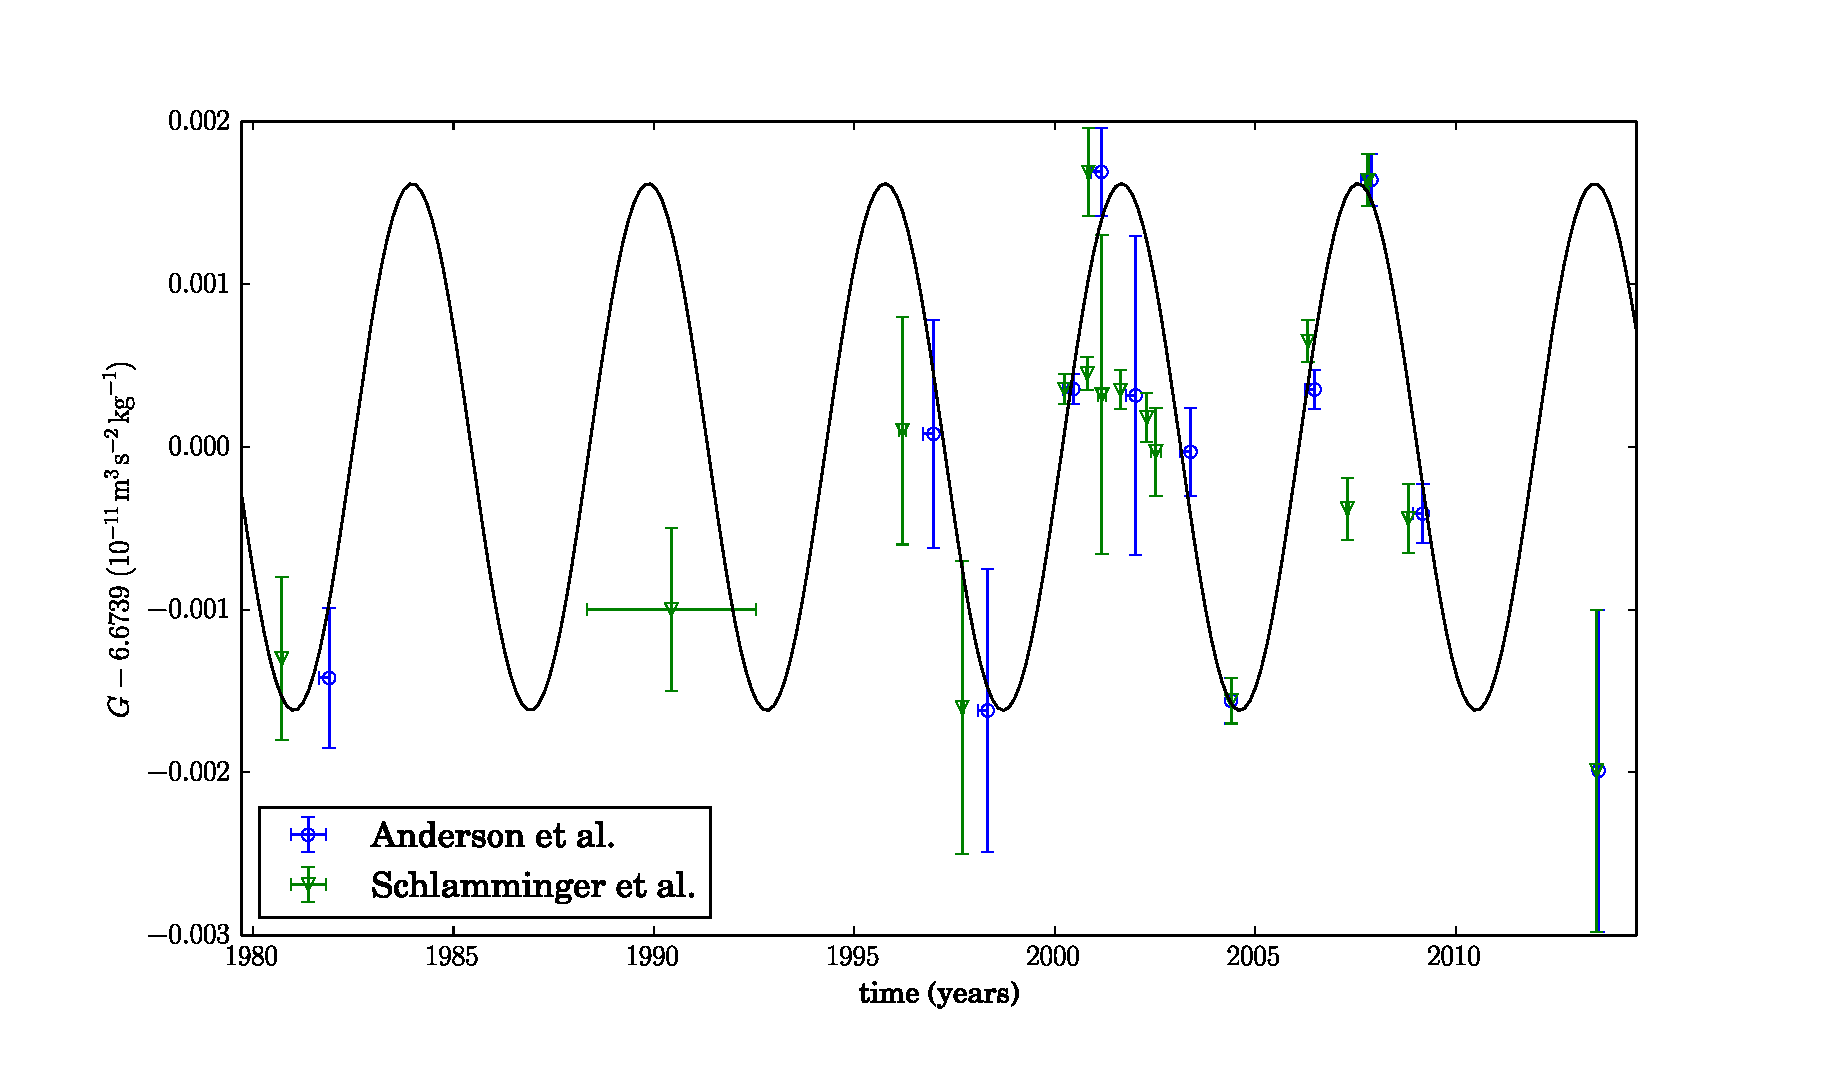
\includegraphics[width=1.0\textwidth]{Gdata}}
 \caption{Experimental values of $G$ from \cite{2015EL....11010002A} (blue circles) and
 \cite{2015arXiv150501774S} (green triangles) as given in table~\ref{tab:Gs}.
 The best fit sinusoid from \cite{2015EL....11010002A} is also
 plotted as a solid black line. Error bars on the times for the blue circles correspond to a half-Gaussian
 before the time point with a standard deviation of 0.25\,years, whilst error bars on the times for the
 green triangles are those given in table~\ref{tab:Gsnew}}
 \label{fig:Gdata}
\end{figure}

Below I define the priors used for calculating the evidence for each of the hypotheses, with the Bayesian
odds ratios comparing the each summarised in table~\ref{tab:results}.

\subsection{Hypothesis 1}

For this hypothesis, $H_1$, there is only one free parameter, $\mu_G$. For $\mu_G$ I choose a prior that is
uniform within a range centred on the sample mean, $\bar{\mu}_G$, given by
\begin{equation}
 p(\mu_G|I) = \begin{cases}
               1/12\sigma_{\mu_G}&\text{ if }\bar{\mu}_G-6\sigma_{\bar{\mu}_G} \leq \mu_G \leq \bar{\mu}_G+6\sigma_{\bar{\mu}_G}, \\
               0&\text{ otherwise},
              \end{cases}
\end{equation}
where $\sigma_{\bar{\mu}_G} = (1/N)[\sum_i^N (d_i - \bar{\mu}_G)^2]^{1/2}$ is the standard error on the mean.
For this hypothesis the model in eq.~(\ref{eq:model}) has $A=0$ and also the unknown Gaussian noise term
$\sigma_{\rm sys}=0$ (i.e.\ $\vect{\theta}_1 = \{\mu_G\}$), so the integral in  eq.~(\ref{eq:jointlike}) to
calculate $Z_1$ is only over $\mu_G$.

\subsection{Hypothesis 2}

For $H_2$ I use the same prior for $\mu_G$ as used in $H_1$, but now also include an unknown Gaussian
noise term, $\sigma_{\rm sys}$, common to all observations. For this I use two different priors; $\sigma_{\rm sys}$
is a scale parameter (it is defined to be only positive) and as such the least informative prior for it
is a Jeffreys prior given by
\begin{equation}
 p(\sigma_{\rm sys}|I) = \begin{cases}
                          \left(\ln{\left( \frac{\sigma_{\rm sys,max}}{\sigma_{\rm sys,min}} \right)\sigma_{\rm sys} }\right)^{-1}&\text{ if }\sigma_{\rm sys,min} \leq \sigma_{\rm sys} \leq \sigma_{\rm sys,max}, \\
                          0&\text{ otherwise},
                         \end{cases}
\end{equation}
where I have set the lower range to be equal to the smallest experimental error, so
$\sigma_{\rm sys,min} = 9.2\,\times\,10^{-16}$, and I have set the upper range to be equal to the
maximum difference between $G$ measurements, so $\sigma_{\rm sys,max} = 3.7\,\times\,10^{-14}$. As a check
that the results are not significantly affected by the prior choice, I have also separately used a uniform prior
on $\sigma_{\rm sys}$, given by
\begin{equation}
 p(\sigma_{\rm sys}|I) = \begin{cases}
               1/\sigma_{\rm sys,max}&\text{ if }0 \leq \sigma_{\rm sys} \leq \sigma_{\rm sys,max}, \\
               0&\text{ otherwise}.
              \end{cases}
\end{equation}
For this hypothesis the model in eq.~(\ref{eq:model}) again has $A=0$, but the integral in 
eq.~(\ref{eq:jointlike}) to calculate $Z_2$ is over $\mu_G$ and $\sigma_{\rm sys}$ (i.e.\ $\vect{\theta}_2 = \{\mu_G, \sigma_{\rm sys}\}$).

\subsection{Hypothesis 3}

For $H_3$ I use the same prior on for $\mu_G$ as used in $H_1$, but now also include the $A$, $P$ and
$\phi_0$ parameters for the sinusoidal model. The sinusoid amplitude, $A$, is a scale parameter, so as with
$\sigma_{\rm sys}$ in $H_2$ I use both a Jeffreys and uniform prior. The Jeffreys prior is given by
\begin{equation}
 p(A|I) = \begin{cases}
               \left(\ln{\left( \frac{A_{\rm max}}{A_{\rm min}} \right)A }\right)^{-1}&\text{ if }A_{\rm min} \leq A \leq A_{\rm max}, \\
               0&\text{ otherwise},
          \end{cases}
\end{equation}
where the lower and upper ranges are set to the same values as for $\sigma_{\rm sys,min}$ and $\sigma_{\rm sys,max}$.
For the uniform prior I have used
\begin{equation}
 p(A|I) = \begin{cases}
               1/A_{\rm max}&\text{ if }0 \leq A \leq A_{\rm max}, \\
               0&\text{ otherwise}.
              \end{cases}
\end{equation}
For the sinusoid period, $P$, I use a uniform prior given by
\begin{equation}
 p(P|I) = \begin{cases}
               1/(P_{\rm max}-P_{\rm max})&\text{ if }P_{\rm min} \leq P \leq P_{\rm max}, \\
               0&\text{ otherwise},
              \end{cases}
\end{equation}
where $P_{\rm min}$ is based on the Nyquist frequency and is twice the minimum time difference between
consecutive measurements, so $P_{\rm min} = 1.4$\,years, and $P_{\rm max}$ is arbitrarily set to be twice
the maximum difference between any consecutive measurements (excluding the initial NIST-82 value), so
$P_{\rm max} = 8.8$\,years, which makes sure that it includes the potential 5.9\,year periodicity. For the
prior on the initial phase, $\phi_0$, I just use a uniform prior over a $2\pi$ range to give
\begin{equation}
 p(\phi_0|I) = \begin{cases}
               1/2\pi&\text{ if }0 \leq \phi_0 \leq 2\pi, \\
               0&\text{ otherwise}.
              \end{cases}
\end{equation}

For this hypothesis $\sigma_{\rm sys} = 0$, but the integral in 
eq.~(\ref{eq:jointlike}) to calculate $Z_3$ is over $\mu_G$, $A$, $P$ and $\phi_0$ (i.e.\ $\{\mu_G,A, P,\phi_0 \}$).

\subsection{Hypothesis 4}

For $H_4$ all the parameters are used, so I use the various priors from the above three hypotheses and
calculate $Z_4$ by integrating over $\mu_G$, $A$, $P$, $\phi_0$ and $\sigma_{\rm sys}$ (i.e.\ $\{\mu_G,A, P,\phi_0,\sigma_{\rm sys} \}$). Both the Jeffreys
and uniform priors for $A$ and $\sigma_{\rm sys}$ are used.

\section{Results}

The odds ratios comparing hypotheses when using the $G$ dataset of \cite{2015EL....11010002A} are summarised in
table~\ref{tab:results}. The odds ratios for the Jeffreys and uniform priors on the scale factor parameters
show only minor differences (they are consistent with a factor of two), so I will only discuss the results from using the Jeffreys prior. It is clear that
hypotheses including extra parameters over that for hypothesis 1 (i.e.\ including a sinusoidal component and/or
and extra unknown noise component) are hugely favoured by factors of $\gtrsim e^{100}$. The two hypotheses, $H_3$
and $H_4$, containing a sinusoidal signal are both approximately equally probable. However, hypothesis 2, just
containing the additional unknown noise term and the unknown offset, is hugely favoured by factors $\sim e^{30}$
over $H_3$ and $H_4$. This suggests that the simple model that variations are just due to an unknown Gaussian
noise term is far more likely to be the cause of the variations than an additional sinusoidal variation.

\begin{table}
\caption{Bayesian odds ratios for the four hypotheses ($i$ represents rows and $j$ represents columns)
when using the data from table~\ref{tab:Gs} equivalent to that used in \cite{2015EL....11010002A}.}
\label{tab:results}
\begin{center}
 \begin{tabular}{c|ccc}
 & \multicolumn{3}{c}{$\mathcal{O}_{ij} = Z_i/Z_j$} \\
 \hline
   & $Z_2$ & $Z_3$ & $Z_4$ \\
  \specialrule{0.25pt}{0.75pt}{0.75pt}
  $Z_1$ & $e^{-132.5}$ & $e^{-102.2}$ & $e^{-102.5}$ \\ 
  $Z_2$ &  & $e^{30.3}$ & $e^{29.9}$ \\
  $Z_3$ &  &  & $0.74$
 \end{tabular}
\end{center}
\end{table}

It is, however, interesting to look at the posterior probability distributions for each of the parameters used
in hypotheses 2, 3 and 4. In fig~\ref{fig:h2} the posterior for $\sigma_{\rm sys}$ shows that this parameter
is peaked well away from zero.
In fig.~\ref{fig:h3}, which shows the posteriors for hypothesis 3, it is clear that in the
posterior for period there is a large spike in probability around the claimed period of 5.9\,years.
A similar spike shows up in fig.~\ref{fig:h4} for hypothesis 4, but is much less pronounced. Despite this we
have shown that the hypotheses containing a sinusoid are hugely less favoured than for hypothesis 2.
This is due to Bayesian model selection naturally applying a penalty for including additional parameters that
to not significantly increase the evidence.

\begin{figure}
 \centerline{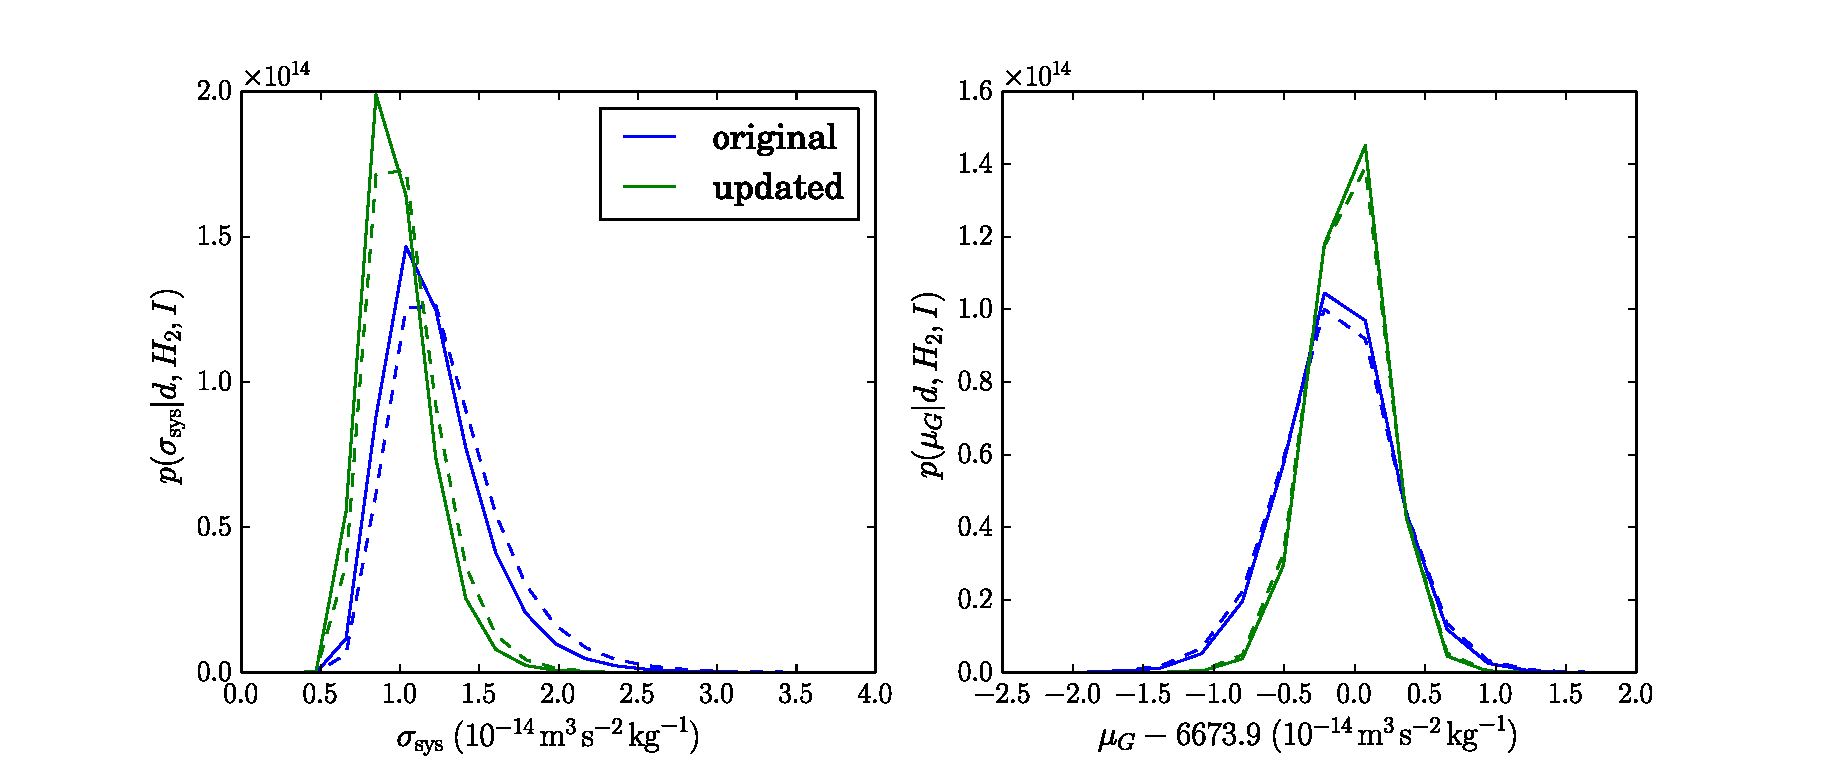
\includegraphics[width=1.0\textwidth]{hypothesis2}}
 \caption{Posterior probability distributions (pdfs) for $\mu_G$ and $\sigma_{\rm sys}$ obtained under hypothesis 2.
 The blue curves represent pdfs using the {\it original} data given in table~\ref{tab:Gs} and the green curves
 represent pdfs using the {\it updated} data given in table~\ref{tab:Gsnew}. The solid curves represent pdfs
 using Jeffreys priors on the scale factor parameters, whilst the dashed curves represent uniform priors on
 these parameters.}
 \label{fig:h2}
\end{figure}

\begin{figure}
 \centerline{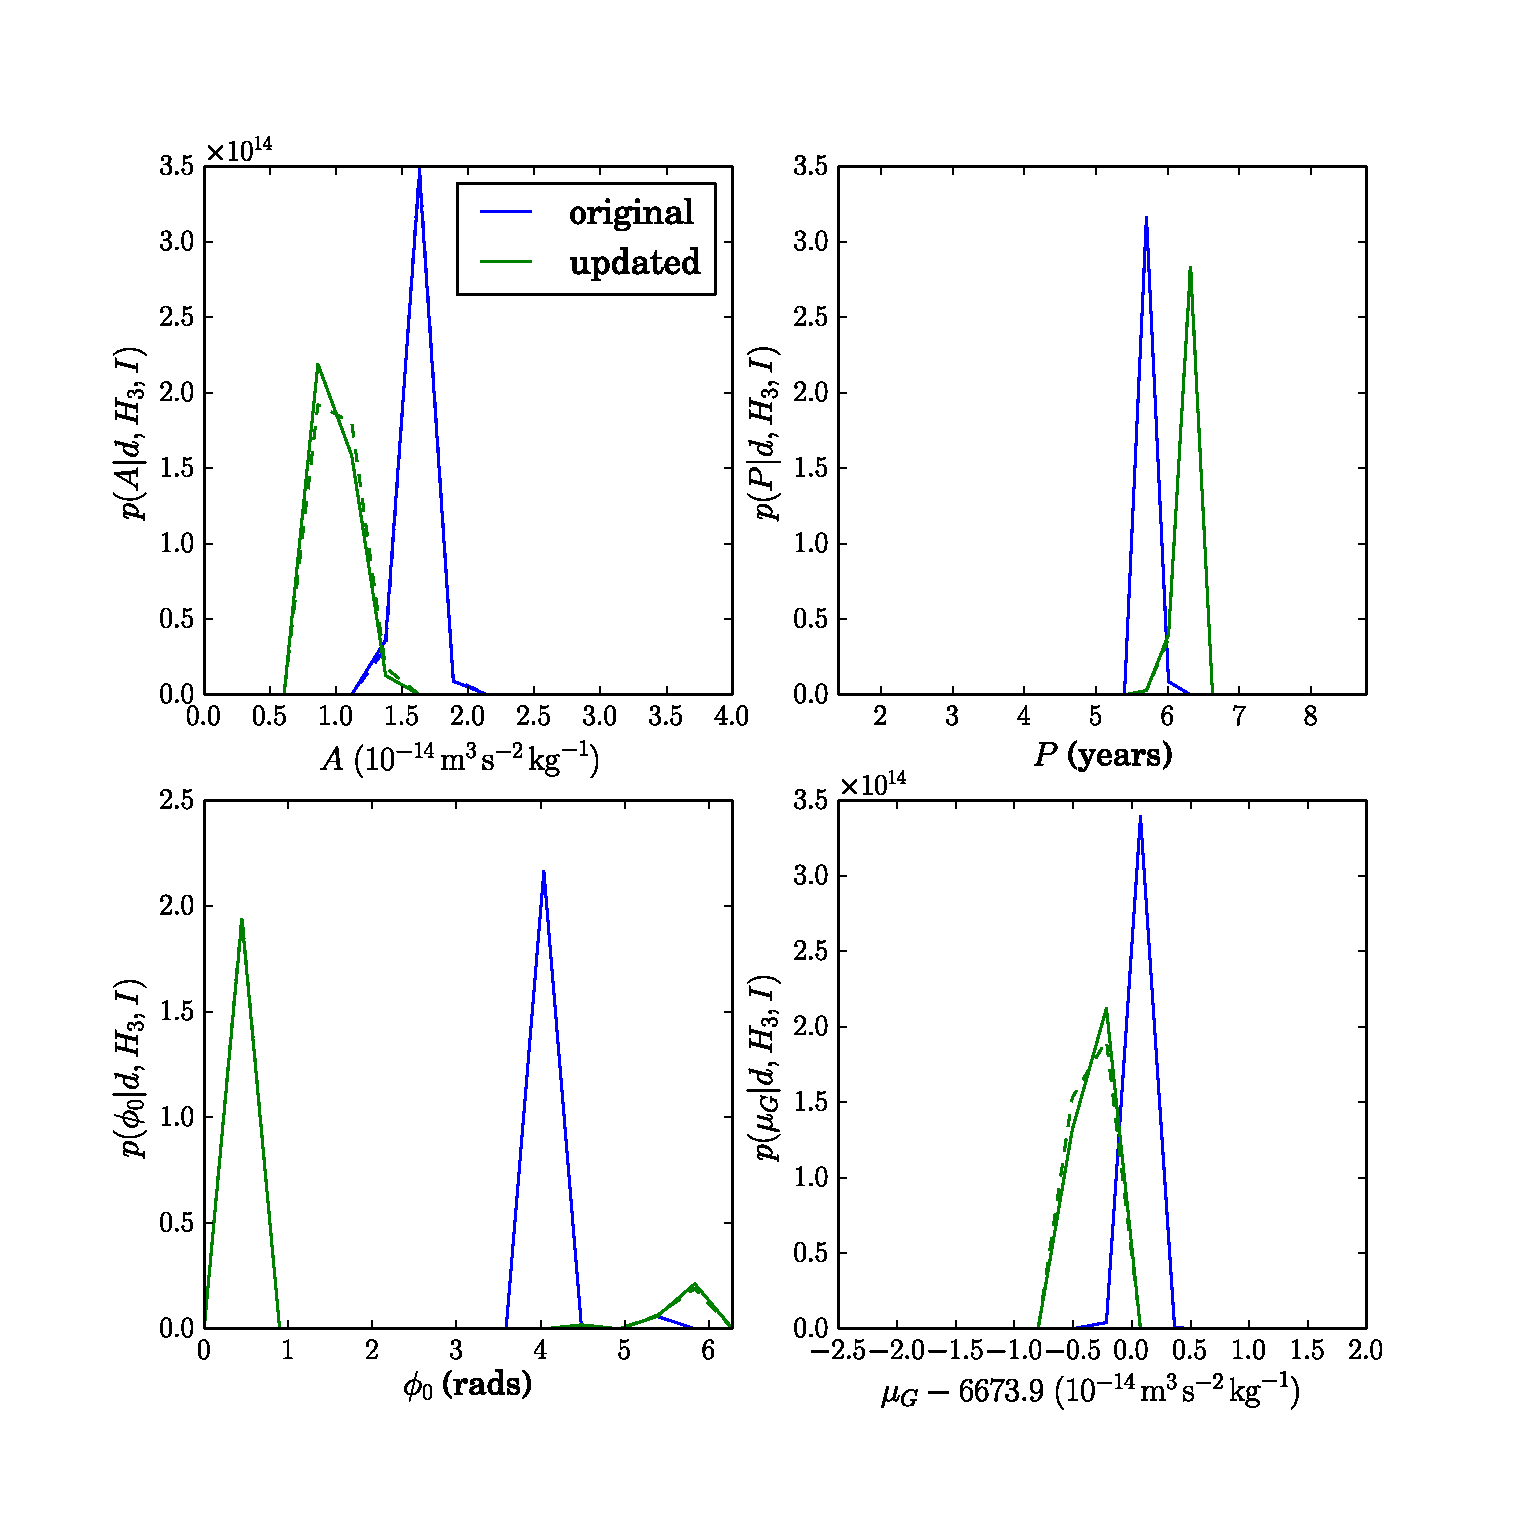
\includegraphics[width=1.0\textwidth]{hypothesis3}}
 \caption{Posterior probability distributions (pdfs) for $\mu_G$, $P$, $A$ and $\phi_0$ obtained under hypothesis 3.}
 \label{fig:h3}
\end{figure}

\begin{figure}
 \centerline{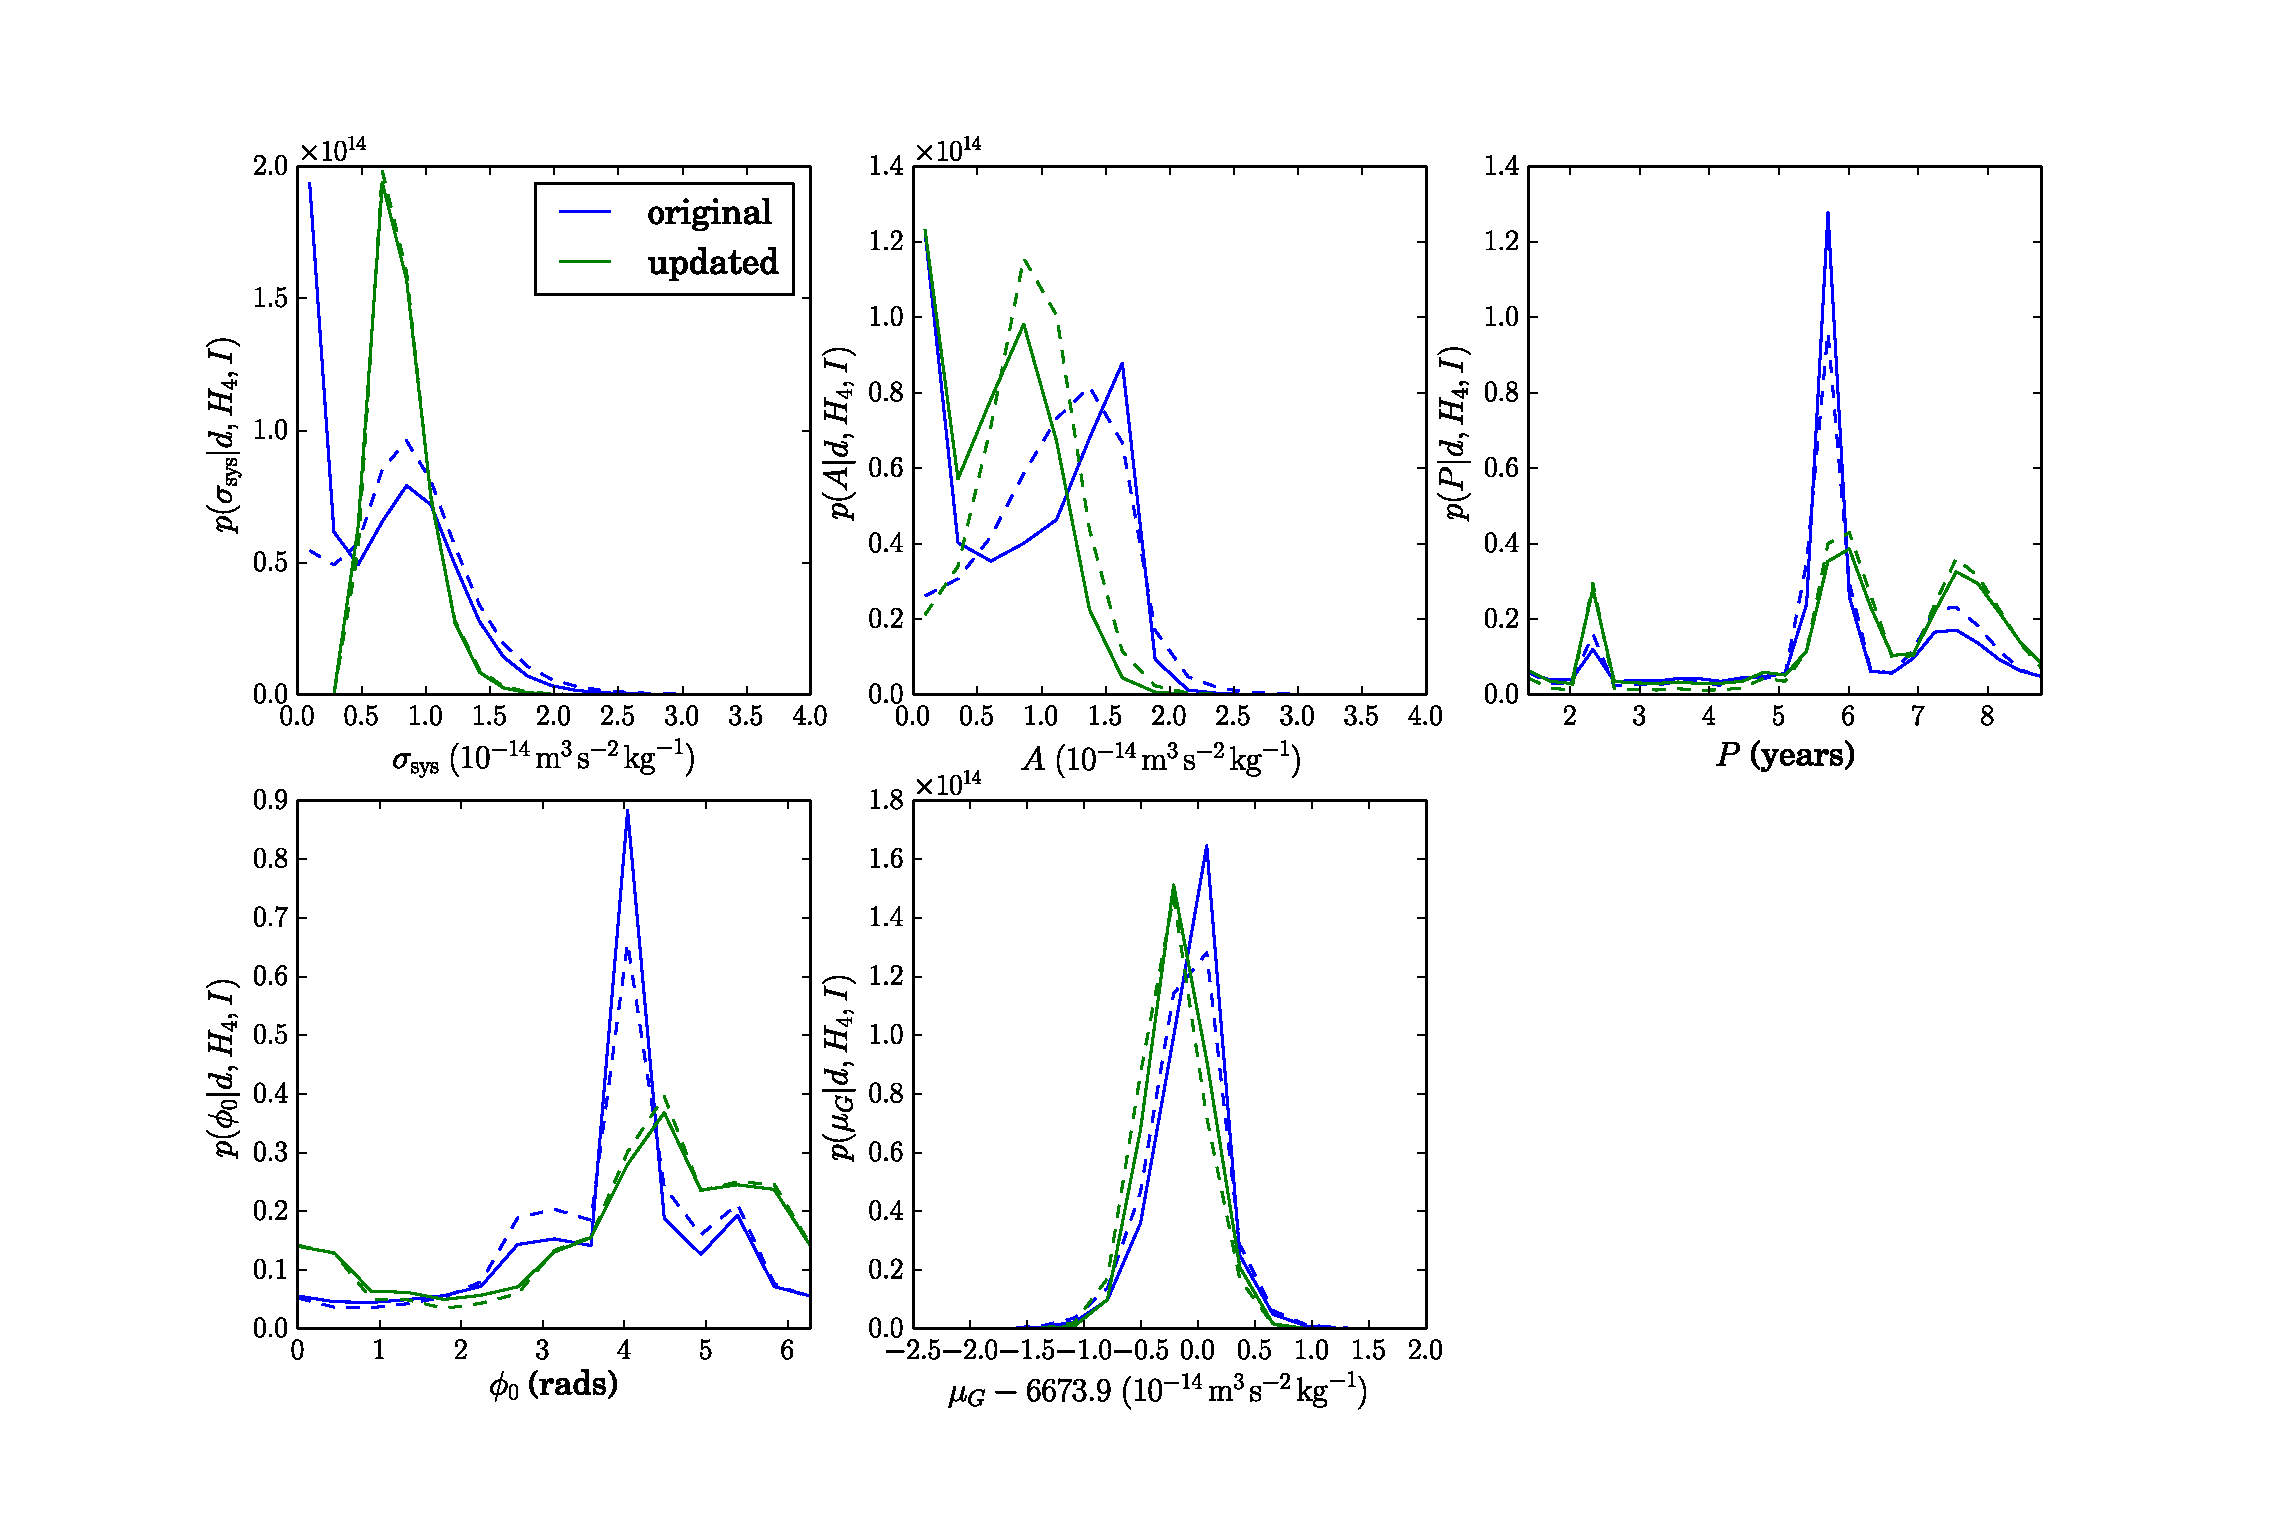
\includegraphics[width=1.0\textwidth]{hypothesis4}}
 \caption{Posterior probability distributions (pdfs) for $\mu_G$, $\sigma_{\rm sys}$, $P$, $A$ and $\phi_0$ obtained under hypothesis 4.}
 \label{fig:h4}
\end{figure}

I have also assessed the significance of the peak for hypothesis 3 by rerunning that analysis 20 times,
but each time randomly shuffling the $G$ values (whilst keeping the measurement times the same). This should remove
any real periodicity in the data. The ratio of each of these evidence values compared to the un-shuffled data are
shown in fig~\ref{fig:ensemble}. Out of these 20 runs there was one time when the hypothesis using the shuffled data
is more favoured than when using the un-shuffled data. The posterior for this case is shown in fig.~\ref{fig:shuf}
showing that seemingly significant spikes in the period can be produced in randomised data.

\begin{figure}
 \centerline{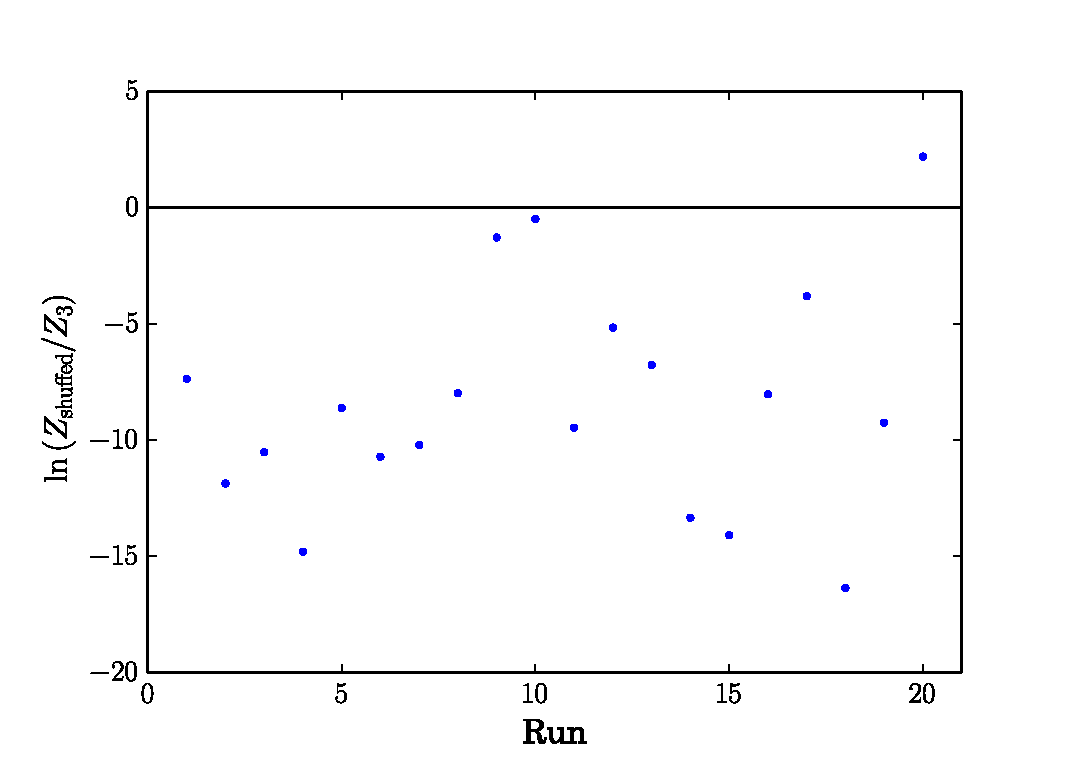
\includegraphics[width=0.6\textwidth]{ensemble}}
 \caption{The odds ratio comparing the evidence for hypothesis 3 when run on randomly shuffled data compared to
 the unshuffled data when using the data from table~\ref{tab:Gs}.}
 \label{fig:ensemble}
\end{figure}

\begin{figure}
 \centerline{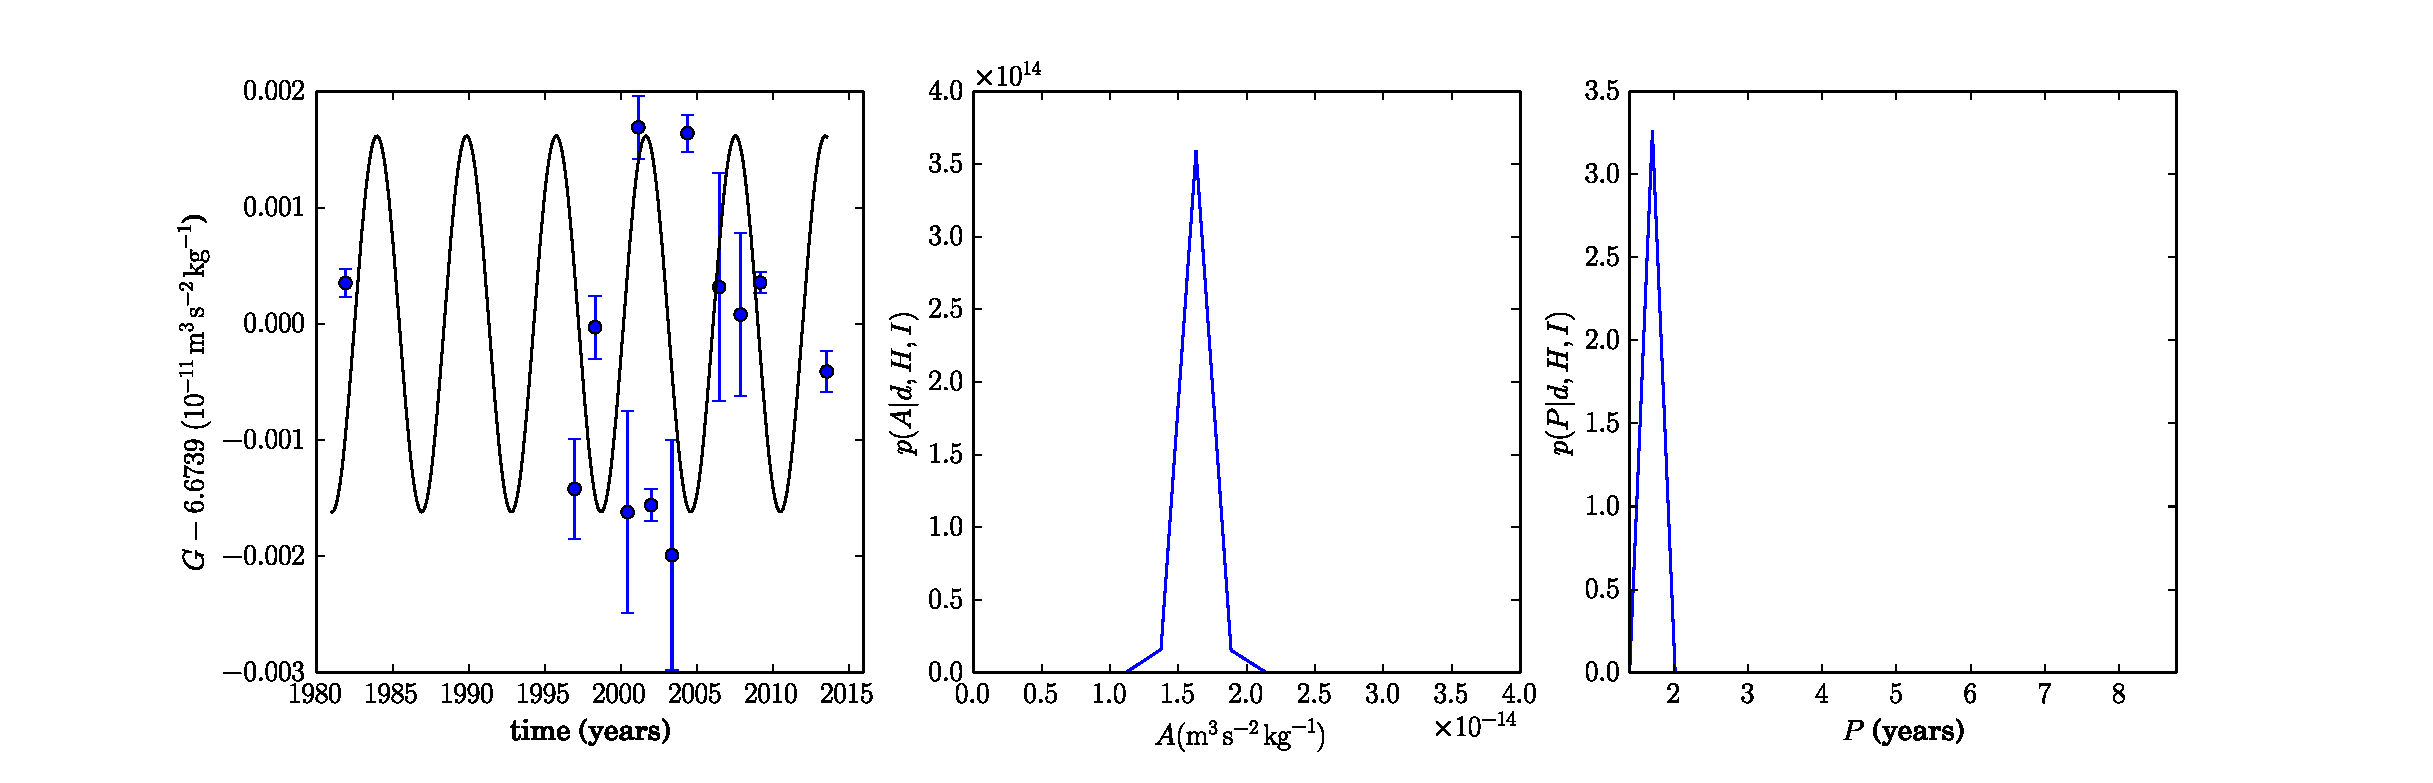
\includegraphics[width=1.0\textwidth]{shuffled}}
 \caption{The shuffled data and the pdfs on $A$ and $P$ for the shuffled data with the largest evidence under
 hypothesis 3. The best fit sinusoid, with a period of 5.9\,years, from \cite{2015EL....11010002A} is also plotted
 as a solid black line.}
 \label{fig:shuf}
\end{figure}

\section{Updated dataset}

Following my initial investigations of the claims of \cite{2015EL....11010002A} Schlamminger, Gundlach and Newman
also examined the claim \cite{2015arXiv150501774S} in particular noting that the experimental times (and also number 
of experimental data used) in the original work are not accurate (e.g. the UZH-06 result that is given as
mid-2006 in table~\ref{tab:Gs} was actually performed in mid-2001). They examined the literature
to compile a more complete list of experiments with information on the actual dates that the experiments were
performed. In table~\ref{tab:Gsnew} I reproduce their information, using their estimates of the mean experiment
date (generally taken as around the centre of any known experimental runs that went into producing the final result)
and an error on that time given as 20\% of the time span over which the experiments were performed.

\begin{table*}
\caption{Experiment times and values of $G$ found in \cite{2015arXiv150501774S}.}
\label{tab:Gsnew}
\begin{center}
 \begin{tabular}{lllr@{}lr@{}l}
  \multicolumn{2}{l}{Experiment} & Date & \multicolumn{2}{c}{$G$} & \multicolumn{2}{c}{time error} \\
  \multicolumn{2}{l}{~} & ~ & \multicolumn{2}{c}{($10^{-11} {\rm m}^3 {\rm sec}^{-2} {\rm kg}^{-1}$)} & \multicolumn{2}{c}{(days)} \\
\toprule
NIST-82 &\cite{PhysRevLett.48.121} & 19 Sep 1980 & 6&.6726 $\pm$ 0.0005 & 8&.4 \\
TR96 &\cite{TR96} & 9 Jun 1990 & 6&.6729 $\pm$ 0.0005 & 767&.0 \\
LANL-97 &\cite{PhysRevLett.78.3047} & 15 Mar 1996 & 6&.6740 $\pm$ 0.0007 & 30&.2 \\
HUST-05 &\cite{PhysRevD.71.127505} & 9 Sep 1997 & 6&.6723 $\pm$ 0.0009 & 14&.4 \\
UWash &\cite{PhysRevLett.85.2869} & 29 Mar 2000 & 6&.674255 $\pm$ 0.000092 & 7&.8 \\
BIPM-01 &\cite{PhysRevLett.87.111101} & 2 Nov 2000 & 6&.67559 $\pm$ 0.00027 & 15&.0 \\
UWup-02 &\cite{UWup} & 6 Mar 2001 & 6&.67422 $\pm$ 0.00098 & 33&.6 \\ 
UZH-06 &\cite{PhysRevD.74.082001} & 21 Aug 2001 & 6&.67425 $\pm$ 0.00012 & 4&.2 \\
MSL-03 &\cite{PhysRevLett.91.201101} & 11 Jul 2002 & 6&.67387 $\pm$ 0.00027 & 45&.0 \\
JILA-10 &\cite{PhysRevLett.105.110801} & 28 May 2004 & 6&.67234 $\pm$ 0.00014 & 5&.0 \\
\specialrule{0.25pt}{0.5pt}{0.5pt}
\multirow{2}{*}{HUST-09} & \multirow{2}{*}{\cite{PhysRevLett.102.240801}} & 20 Apr 2007 & 6&.67352 $\pm$ 0.00019 & 12&.0 \\
 & & 27 Oct 2008 & 6&.67346 $\pm$ 0.00021 & 7&.8 \\
\specialrule{0.25pt}{0.5pt}{0.5pt}
BIPM-13 &\cite{PhysRevLett.111.101102,PhysRevLett.113.039901} & 25 Oct 2007 & 6&.67554 $\pm$ 0.00016 & 27&.6 \\
\specialrule{0.25pt}{0.5pt}{0.5pt}
\multirow{3}{*}{UCI-14} & \multirow{3}{*}{\cite{UCI}} & 23 Oct 2000 & 6&.67435 $\pm$ 0.0001 & 7&.6 \\
 & & 18 Apr 2002 & 6&.67408 $\pm$ 0.00015 & 9&.6 \\
 & & 26 Apr 2006 & 6&.67455 $\pm$ 0.00013 & 7&.2 \\
\specialrule{0.25pt}{0.5pt}{0.5pt}
LENS-14 &\cite{2014Natur.510..518R} & 8 Jul 2013 & 6&.67191 $\pm$ 0.00099 & 1&.4
\end{tabular}
\end{center}
\end{table*}

I have reanalysed this new dataset for each of the four hypotheses. When integrating over the
time error from eq.~(\ref{eq:margT}) I have set $X=Y=2.5$, so that the the prior range is symmetric around the
mean experiment time with the standard deviations using the values given in table~\label{tab:Gsnew}.
For all other parameters I have used the same prior ranges as before.
The Bayesian odds ratios for each of these cases are given in table~\ref{tab:newresults} from which it can
be seen that hypothesis 2 is still favoured over all other hypotheses by a huge amount. However, hypothesis 3
is now hugely disfavoured over hypothesis 4, i.e.\ just including a sinusoid, but adding no additional noise
term does far worse at fitting the data than also including the noise term.

\begin{table}
\caption{Bayesian odds ratios for the four hypotheses ($i$ represents rows and $j$ represents columns)
when using the data from table~\ref{tab:Gsnew} from \cite{2015arXiv150501774S}.}
\label{tab:newresults}
\begin{center}
 \begin{tabular}{l|ccc}
 & \multicolumn{3}{c}{$\mathcal{O}_{ij} = Z_i/Z_j$} \\
 \hline
   & $Z_2$ & $Z_3$ & $Z_4$ \\
  \specialrule{0.25pt}{0.75pt}{0.75pt}
  $Z_1$ & $e^{-140.2}$ & $e^{-65.8}$ & $e^{-110.3}$ \\
  $Z_2$ & & $e^{74.4}$ & $e^{29.9}$  \\
  $Z_3$ & & & $e^{-44.5}$
 \end{tabular}
\end{center}
\end{table}

\section{Conclusions}

I have reanalysed the data consisting of measurements of Newton's gravitational constant $G$ from
\cite{2015EL....11010002A} and \cite{2015arXiv150501774S}. In \cite{2015EL....11010002A} there was claimed
evidence for a periodic component with a period of 5.9\,years that was very strongly correlated with the
period of changes of the length of the day. It was not suggested that $G$ was actually varying on these
timescales, but rather that there could be some systematic effect on the measurement process that was
correlated with the mechanism that leads to the variation in the length of the day.

Using Bayesian model selection, and four different hypotheses to describe the variations in the data, and including
uncertainties on the experimental times, I have found that the best model to describe the data is one in which
there is an additional common unknown Gaussian noise term on top of the oberserved experimental values. This is 
favoured over a model also containing a sinusoidal term by factors of $\gtrsim e^{30}$. I also find that periodic
signals can easily be found in random permutations of the data suggesting that the observed periodicity seen in
\cite{2015EL....11010002A} is just a random artifact of the data.

I note that if there were very good a priori reasons to expect a periodic component in the data, and a known
period range and/or initial phase (i.e.\ if there were a good reason why the the mechanism leading to changes in the
length of the day could couple into measurements of $G$), then the evidence in favour models containing a periodic
signal would dramatically increase. However, without such prior knowledge using such a constraint would strongly bias
us.

\acknowledgements

I would like to thank Prof.\ J.\ Faller for useful discussions, Prof.\ C.\ Speake for putting me in contact with
Dr.\ S.\ Schlamminger, and Dr.\ Schlamminger for providing me with a data file of their compiled $G$ measurements.
I am funded by the STFC under grant ST/L000946/1. The code for this analysis can be found at \url{https://github.com/mattpitkin/periodicG}.

\bibliographystyle{eplbib}
\bibliography{comment}

\end{document}